% Mẫu tín hiệu có biên độ x = 0.506683, vẽ lại từ ảnh tham chiếu.
% Chèn bằng % Mẫu tín hiệu có biên độ x = 0.506683, vẽ lại từ ảnh tham chiếu.
% Chèn bằng % Mẫu tín hiệu có biên độ x = 0.506683, vẽ lại từ ảnh tham chiếu.
% Chèn bằng % Mẫu tín hiệu có biên độ x = 0.506683, vẽ lại từ ảnh tham chiếu.
% Chèn bằng \input{figures/bai_tap_luong_tu_hoa_2.tex}; cần gói tikz.
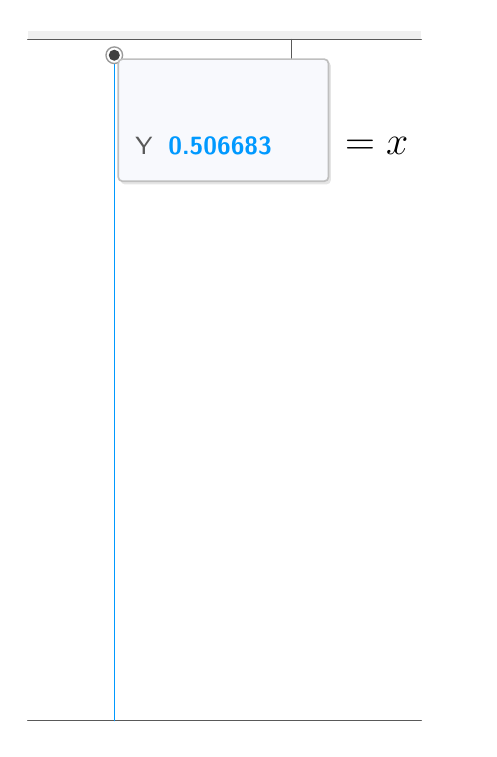
\begin{tikzpicture}[
    x=1cm,
    y=1cm,
    line cap=round,
    line join=round
]
    \definecolor{quantizationsampletwo}{RGB}{0, 153, 255}
    \definecolor{quantizationtipfill}{RGB}{248, 249, 253}

    % Giữ dáng hình hẹp và cao như ảnh gốc.
    \path[use as bounding box] (0, -0.10) rectangle (5.60, 8.80);

    % Hai đường ngang giới hạn đồ thị và vạch chia phía trên.
    \fill[black!6] (0, 8.65) rectangle (5, 8.76);
    \draw[black!65, line width=0.45pt] (0, 8.65) -- (5, 8.65);
    \draw[black!65, line width=0.45pt] (3.35, 8.65) -- (3.35, 8.39);
    \draw[black!65, line width=0.45pt] (0, 0) -- (5, 0);

    % Vạch mẫu màu xanh và điểm được chọn ở đầu vạch.
    \draw[quantizationsampletwo, line width=0.5pt]
        (1.10, 0) -- (1.10, 8.45);
    \draw[draw=black!40, fill=white, line width=0.5pt]
        (1.10, 8.45) circle[radius=3pt];
    \fill[black!75] (1.10, 8.45) circle[radius=2pt];

    % Hộp đọc biên độ: giữ khoảng trống phía trên như trong ảnh.
    \path[fill=black!10, rounded corners=1.5pt]
        (1.18, 6.81) rectangle (3.85, 8.37);
    \path[draw=black!25, fill=quantizationtipfill,
        line width=0.6pt, rounded corners=1.5pt]
        (1.15, 6.85) rectangle (3.82, 8.40);
    \node[anchor=west, inner sep=0pt,
        font=\sffamily\small, text=black!65]
        at (1.36, 7.30) {Y};
    \node[anchor=west, inner sep=0pt,
        font=\sffamily\small\bfseries, text=quantizationsampletwo]
        at (1.78, 7.30) {0.506683};

    % Chú thích bên cạnh giá trị biên độ: dấu bằng và chữ x màu đen.
    \node[anchor=west, inner sep=0pt, font=\Large, text=black]
        at (4.02, 7.30) {$=x$};
\end{tikzpicture}
; cần gói tikz.
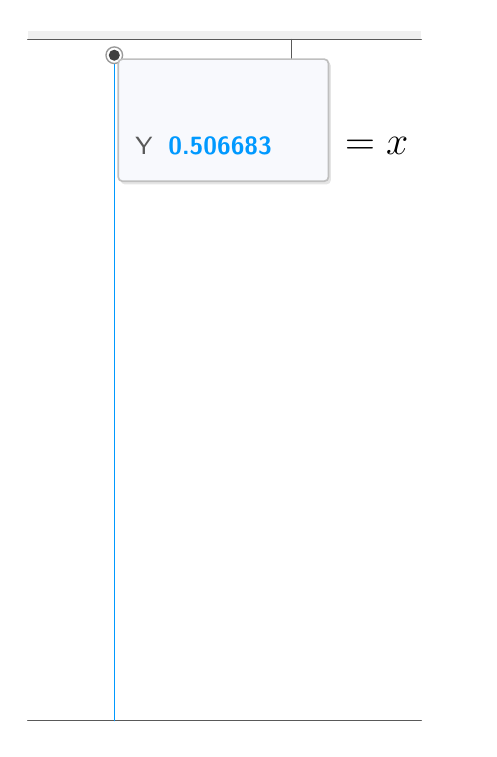
\begin{tikzpicture}[
    x=1cm,
    y=1cm,
    line cap=round,
    line join=round
]
    \definecolor{quantizationsampletwo}{RGB}{0, 153, 255}
    \definecolor{quantizationtipfill}{RGB}{248, 249, 253}

    % Giữ dáng hình hẹp và cao như ảnh gốc.
    \path[use as bounding box] (0, -0.10) rectangle (5.60, 8.80);

    % Hai đường ngang giới hạn đồ thị và vạch chia phía trên.
    \fill[black!6] (0, 8.65) rectangle (5, 8.76);
    \draw[black!65, line width=0.45pt] (0, 8.65) -- (5, 8.65);
    \draw[black!65, line width=0.45pt] (3.35, 8.65) -- (3.35, 8.39);
    \draw[black!65, line width=0.45pt] (0, 0) -- (5, 0);

    % Vạch mẫu màu xanh và điểm được chọn ở đầu vạch.
    \draw[quantizationsampletwo, line width=0.5pt]
        (1.10, 0) -- (1.10, 8.45);
    \draw[draw=black!40, fill=white, line width=0.5pt]
        (1.10, 8.45) circle[radius=3pt];
    \fill[black!75] (1.10, 8.45) circle[radius=2pt];

    % Hộp đọc biên độ: giữ khoảng trống phía trên như trong ảnh.
    \path[fill=black!10, rounded corners=1.5pt]
        (1.18, 6.81) rectangle (3.85, 8.37);
    \path[draw=black!25, fill=quantizationtipfill,
        line width=0.6pt, rounded corners=1.5pt]
        (1.15, 6.85) rectangle (3.82, 8.40);
    \node[anchor=west, inner sep=0pt,
        font=\sffamily\small, text=black!65]
        at (1.36, 7.30) {Y};
    \node[anchor=west, inner sep=0pt,
        font=\sffamily\small\bfseries, text=quantizationsampletwo]
        at (1.78, 7.30) {0.506683};

    % Chú thích bên cạnh giá trị biên độ: dấu bằng và chữ x màu đen.
    \node[anchor=west, inner sep=0pt, font=\Large, text=black]
        at (4.02, 7.30) {$=x$};
\end{tikzpicture}
; cần gói tikz.
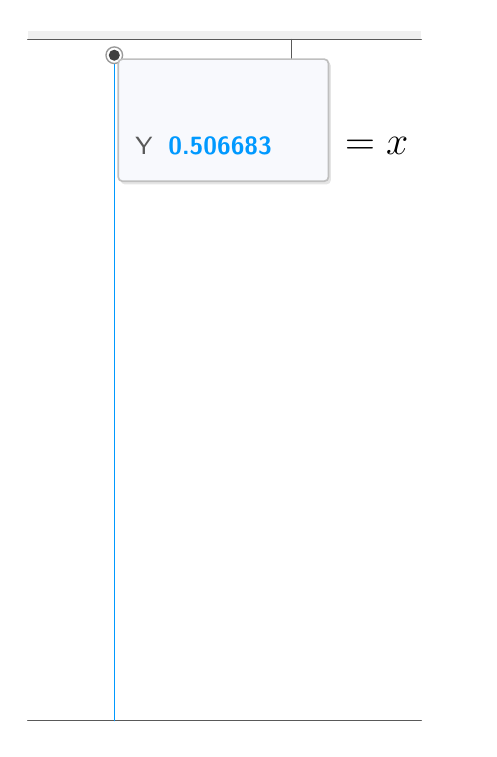
\begin{tikzpicture}[
    x=1cm,
    y=1cm,
    line cap=round,
    line join=round
]
    \definecolor{quantizationsampletwo}{RGB}{0, 153, 255}
    \definecolor{quantizationtipfill}{RGB}{248, 249, 253}

    % Giữ dáng hình hẹp và cao như ảnh gốc.
    \path[use as bounding box] (0, -0.10) rectangle (5.60, 8.80);

    % Hai đường ngang giới hạn đồ thị và vạch chia phía trên.
    \fill[black!6] (0, 8.65) rectangle (5, 8.76);
    \draw[black!65, line width=0.45pt] (0, 8.65) -- (5, 8.65);
    \draw[black!65, line width=0.45pt] (3.35, 8.65) -- (3.35, 8.39);
    \draw[black!65, line width=0.45pt] (0, 0) -- (5, 0);

    % Vạch mẫu màu xanh và điểm được chọn ở đầu vạch.
    \draw[quantizationsampletwo, line width=0.5pt]
        (1.10, 0) -- (1.10, 8.45);
    \draw[draw=black!40, fill=white, line width=0.5pt]
        (1.10, 8.45) circle[radius=3pt];
    \fill[black!75] (1.10, 8.45) circle[radius=2pt];

    % Hộp đọc biên độ: giữ khoảng trống phía trên như trong ảnh.
    \path[fill=black!10, rounded corners=1.5pt]
        (1.18, 6.81) rectangle (3.85, 8.37);
    \path[draw=black!25, fill=quantizationtipfill,
        line width=0.6pt, rounded corners=1.5pt]
        (1.15, 6.85) rectangle (3.82, 8.40);
    \node[anchor=west, inner sep=0pt,
        font=\sffamily\small, text=black!65]
        at (1.36, 7.30) {Y};
    \node[anchor=west, inner sep=0pt,
        font=\sffamily\small\bfseries, text=quantizationsampletwo]
        at (1.78, 7.30) {0.506683};

    % Chú thích bên cạnh giá trị biên độ: dấu bằng và chữ x màu đen.
    \node[anchor=west, inner sep=0pt, font=\Large, text=black]
        at (4.02, 7.30) {$=x$};
\end{tikzpicture}
; cần gói tikz.
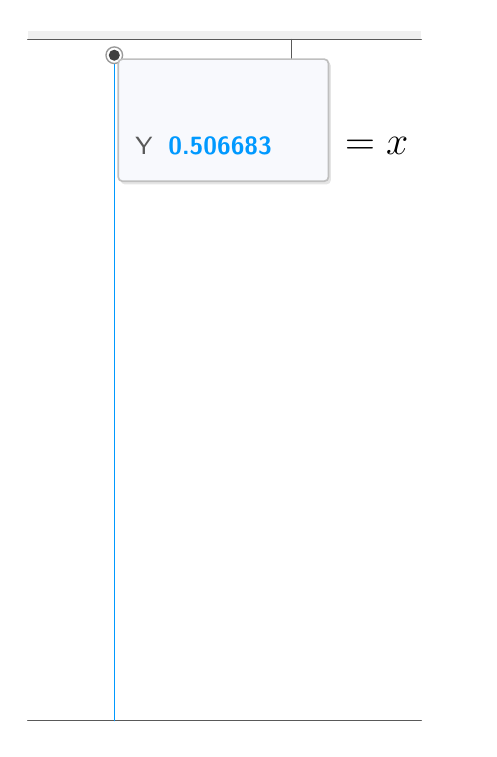
\begin{tikzpicture}[
    x=1cm,
    y=1cm,
    line cap=round,
    line join=round
]
    \definecolor{quantizationsampletwo}{RGB}{0, 153, 255}
    \definecolor{quantizationtipfill}{RGB}{248, 249, 253}

    % Giữ dáng hình hẹp và cao như ảnh gốc.
    \path[use as bounding box] (0, -0.10) rectangle (5.60, 8.80);

    % Hai đường ngang giới hạn đồ thị và vạch chia phía trên.
    \fill[black!6] (0, 8.65) rectangle (5, 8.76);
    \draw[black!65, line width=0.45pt] (0, 8.65) -- (5, 8.65);
    \draw[black!65, line width=0.45pt] (3.35, 8.65) -- (3.35, 8.39);
    \draw[black!65, line width=0.45pt] (0, 0) -- (5, 0);

    % Vạch mẫu màu xanh và điểm được chọn ở đầu vạch.
    \draw[quantizationsampletwo, line width=0.5pt]
        (1.10, 0) -- (1.10, 8.45);
    \draw[draw=black!40, fill=white, line width=0.5pt]
        (1.10, 8.45) circle[radius=3pt];
    \fill[black!75] (1.10, 8.45) circle[radius=2pt];

    % Hộp đọc biên độ: giữ khoảng trống phía trên như trong ảnh.
    \path[fill=black!10, rounded corners=1.5pt]
        (1.18, 6.81) rectangle (3.85, 8.37);
    \path[draw=black!25, fill=quantizationtipfill,
        line width=0.6pt, rounded corners=1.5pt]
        (1.15, 6.85) rectangle (3.82, 8.40);
    \node[anchor=west, inner sep=0pt,
        font=\sffamily\small, text=black!65]
        at (1.36, 7.30) {Y};
    \node[anchor=west, inner sep=0pt,
        font=\sffamily\small\bfseries, text=quantizationsampletwo]
        at (1.78, 7.30) {0.506683};

    % Chú thích bên cạnh giá trị biên độ: dấu bằng và chữ x màu đen.
    \node[anchor=west, inner sep=0pt, font=\Large, text=black]
        at (4.02, 7.30) {$=x$};
\end{tikzpicture}
